\chapter{Segmentation} \label{ch:segmentation}

We discuss how we use the Frangi as a prefilter and discuss several different segmentation strategies based upon our Frangi-filtered result. We will compare these methods to an unrelated segmentation strategy, the ISODATA threshold. First, we define some standard quantitative measures of success for segmentation methods.


\section{Binary Classifications, Scoring Methods, and the Confusion Matrix}

We wish to come up wish a means of gauging the success of an arbitrary segmentation and will adopt a binary classification model to do so.
We end up with a boolean matrix the size of the image, and compare it to the ground truth, the trace, and then compare them to get the number of true positives (TP), true negatives (TN), false positives (FP), and false negatives (FN). We demonstrate these four labels visually with a confusion matrix, as in \cref{fig:sample-confusion}.
% The lighter gray represents true negatives (TN), red represents false negatives (FN), blue represents false positives (FP), and black represents true positives. The darkest gray are is the background mask (pixels are not considered at all in gauging the success of segmentation).
 
\begin{figure}
  \centering
  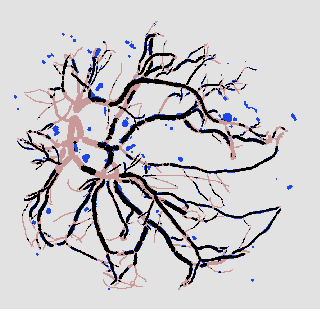
\includegraphics[height=0.3\textheight]{example_confusion_small}
  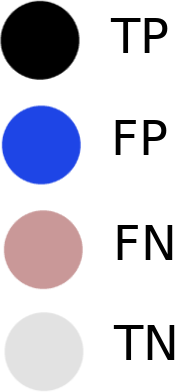
\includegraphics[height=0.12\textheight]{confusion_legend}
  \caption{Sample confusion matrix}
  \label{fig:sample-confusion}
\end{figure}

Although there are many measures to gauge the success of binary classification, we will focus on two that we find particularly illustrative. The first is precision, given by

\begin{equation}
\label{eq:precision}
\textrm{precision} \;=\; \frac{TP}{TP+FP}
\end{equation}
\noindent and the second is the Matthews Correlation Constant (MCC), given by

\begin{equation} \label{eq:MCC}
MCC = \frac{TP\times TN - FP \times FN}{\sqrt{ (TP + FP)(TP+FN)(TN+FP)(TN+FN)}}
\end{equation}
\noindent where precision is a ratio between 0\% and 100\% and the MCC is a measure between -1 and 1. Precision (or positive predictive power) is defined as the ratio between how many pixels were labeled correctly (true positives) and all pixels labeled positive (either correctly or incorrectly). This is a useful score for us--if we are using Frangi as a prefiltering for a more robust technique, then we would rather provide an incomplete starting point, rather than an inaccurate one. Precision therefore does an okay job of representing that scenario: we are not penalized for what we do not label as true, as long as our reports of true are correct.

Of course, we cannot rely on precision as our sole quantitative factor alone--we could simply return everything negative and receive a perfect score of 100\% precision. Therefore we will gauge that measure with that of the MCC \autocite{mcc-original-paper}. The main advantage of the MCC is that it is well balanced no matter what the size of the two classes are, and will only be high if the approximation scores well against both labels. A score of $1.0$ means the approximation is 100\% correct, a score of $-1.0$ means that everything is completely incorrect, and a score of $0$ means that the test performs only as well as random guessing. In our analysis, we will consider both the MCC and precision of a particular segmentation simultaneously. We would like an MCC score as high as possible, but will contextually settle for a lower score as long as the approximation is sufficiently precise.

One final point about these measures is that we have decided to report their scores only within the placental plate, rather than the entire rectangular image. Since the area outside of plate is masked from consideration, those points will be true negatives no matter what, and we don't want these points to artificially inflate our score. That being said, we do currently concede one part right now: we will also mask an area around the umbilical cord insertion point, as the large amount of noise here will mean that our scores are artificially low. We would like to remove these areas, but for now we will simply not score them. 

\section{Postprocessing Techniques}
Here we develop four relatively straightforward methods of postprocessing the multiscale Frangi output to obtain an actual PCSVN extraction. Again, we stress that the Frangi filter itself does not produce a segmentation itself. In fact, Frangi in his original paper \autocite{frangi-paper} refrained from any explicit analysis of the Frangi score apart from taking the maximum across all scales. Still, we wish to demonstrate some immediate methods of postprocessing these samples in order to illustrate the usefulness of this optimized Frangi filter. 


\subsection{Method A: Fixed Threshold}
Like \textcite{huynh2013filter}, we consider a thresholded \Vmax{} as a crude segmentation.
In the fixed threshold method, we choose some threshold $\alpha$ and we say that a pixel $(x,y)$ of the image corresponds to a vessel if
$\Vmax >  \alpha$. This $\alpha$, as noted above, is unfortunately highly dependent on the image domain, and this merging method will tend to happily allow noise generated from scales that are too large or too small if $\Sigma$ is not chosen correctly. We would hope that some normalization of our data set would permit a single choice of $\alpha$ across all samples, but unfortunately we cannot seem to guarantee this. Without prior knowledge of an appropriate choice of $\alpha$, we may have to simply select $\alpha$ by trial and error.

 Another issue with this is the individual scales of the Frangi filter in the extreme cases are not known to scale--although Lindeberg introduced a normalization factor based on the scale to apply to the derivatives, we do not know of an optimal factor to use.

Unfortunately, even with our ``rescaled'' Frangi filter, this $\alpha$ cannot be picked without regard for the particular image domain. Equally problematic, we cannot guarantee that the Frangi filter will decay as our scale exceeds the the bounds where structure is expected to be found.


%\begin{equation}
%{\VSigma}_{\alpha}(x_0,y_0) = \begin{cases}
%1 & \textrm{if}\quad \Vmax(x,y) \; \ge\;  \alpha \\
%0 & \textrm{else}
%\end{cases}  \quad , \; \alpha > 0
%\; \textrm{for}\;\alpha\;\textrm{fixed}.
%\end{equation}

If we insist on such a performing such a thresholding, the ``correct'' choice of $\alpha$ unfortunately seems to depend on the image domain, so user intervention when dealing with the problem domain seems to be the best strategy. A more sincere use of thresholding might be to choose a relatively high threshold, and then use the result for a further technique.
We will discuss alternatives methods of aggregating results from our multiscale method, as well as optimal values for parameters and scales. As a final note, we admit that any future extensions of this work should not hold too much stock in this thresholded result. Analyzing the raw vesselness score \cref{eq:Vmax}, or even the un-merged scale-wise scores \cref{eq:VSigma}, would be far more rewarding.
 
\subsection{Method B: Scalewise Percentile Based Merging}

There is an alternative method of thresholding which avoids the domain-dependent selection of a fixed threshold $\alpha$ altogether. Instead, we could simply select the highest scores from each responses: we calculate a high percentile score and threshold at that value. Due to the large number of zeros outputted by the filter, we opt instead to take the $p$th percentile of only nonzero values of each $\Vsigma$. 
We briefly demonstrate this in \cref{fig:qthresh_demo} on a particularly well-behaved sample. The idea behind percentile-based merging is beneficial for multiscale methods. At each scale, we would like to assume that there is \textit{some} curvilinear content that could be identified. With that in mind, we could simply accept from each scales scores in a very high percentile. We chose for our demonstration a fairly large percentile, $95$, and furthermore bolster this by requiring that any selected pixels be in the 95th percentile of nonzero and unmasked pixels--otherwise the average is artificially low due to the large background and pixels with zero Frangi score. The use of percentiles removes dependence of picking a particular threshold on the problem, while allowing the most prominent features to emerge at each scale.

\begin{figure} \centering
	\subfloat[grayscale image]{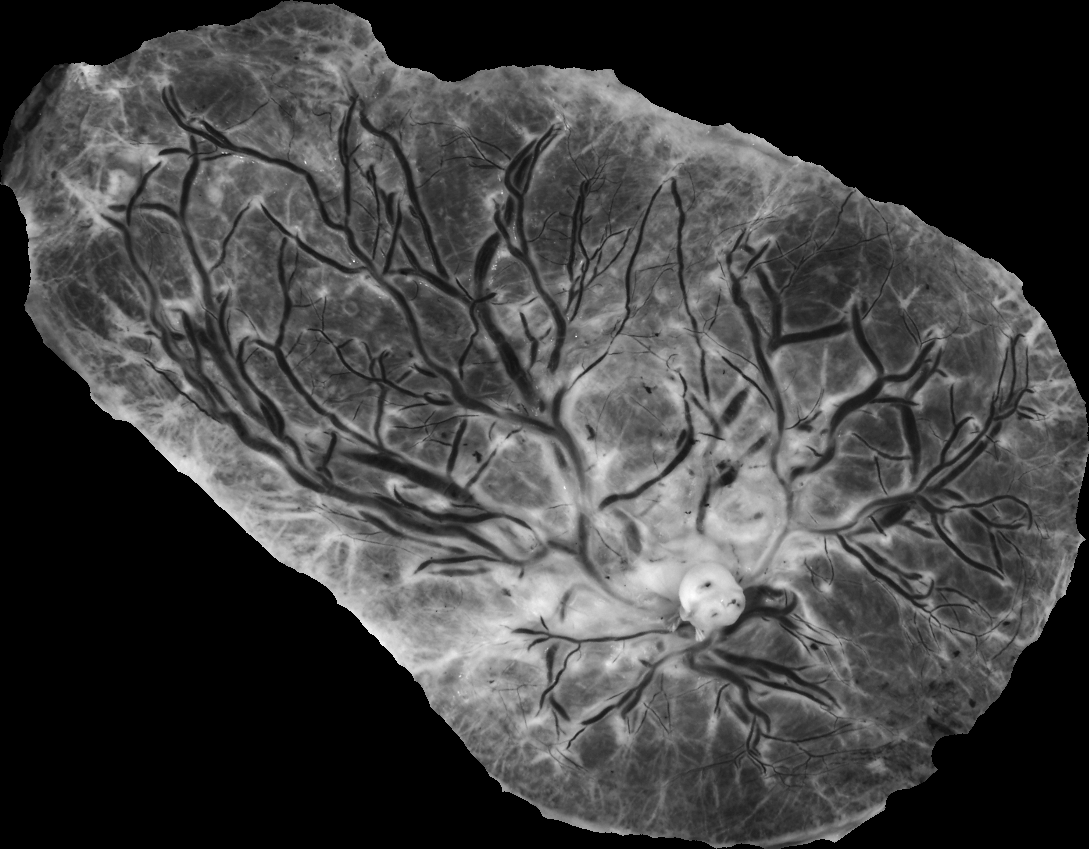
\includegraphics[width=0.48\linewidth]{qthresh_demo_img}}
	\subfloat[\Vmax]{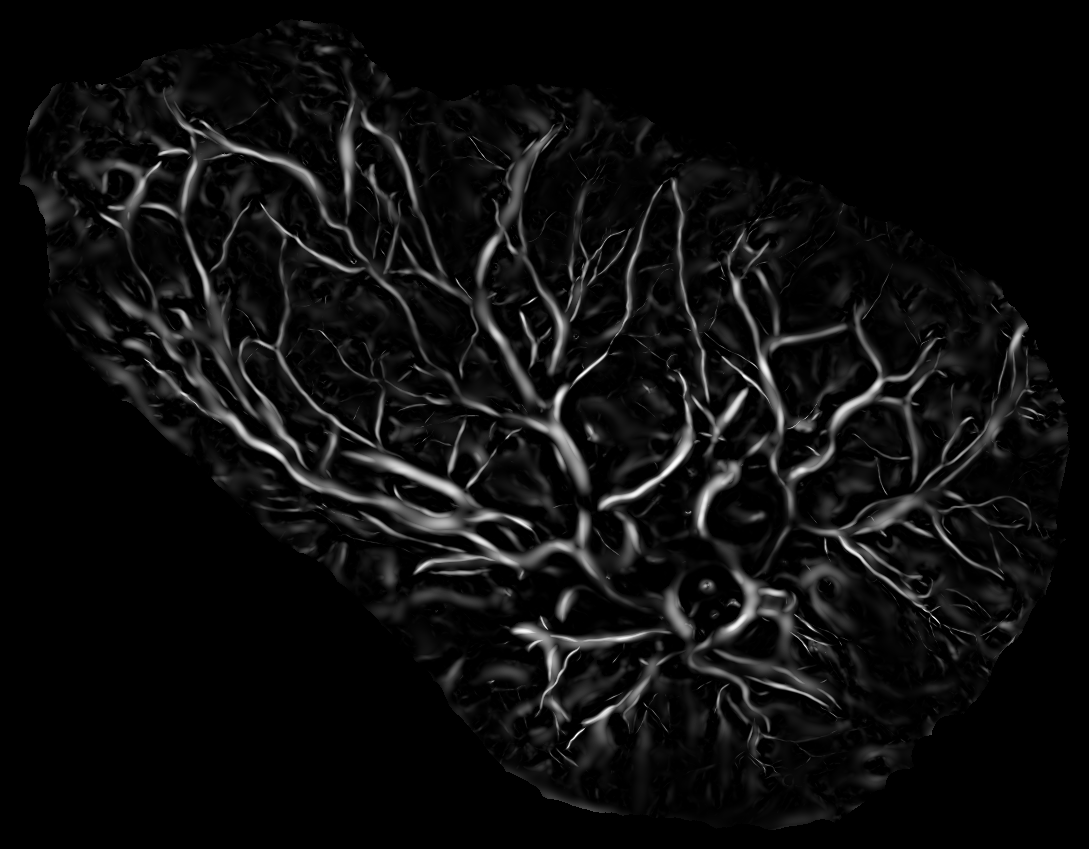
\includegraphics[width=0.48\linewidth]{qthresh_demo_Fmax}} \\
	\subfloat[scalewise percentile filtering ($p=95$)]{
		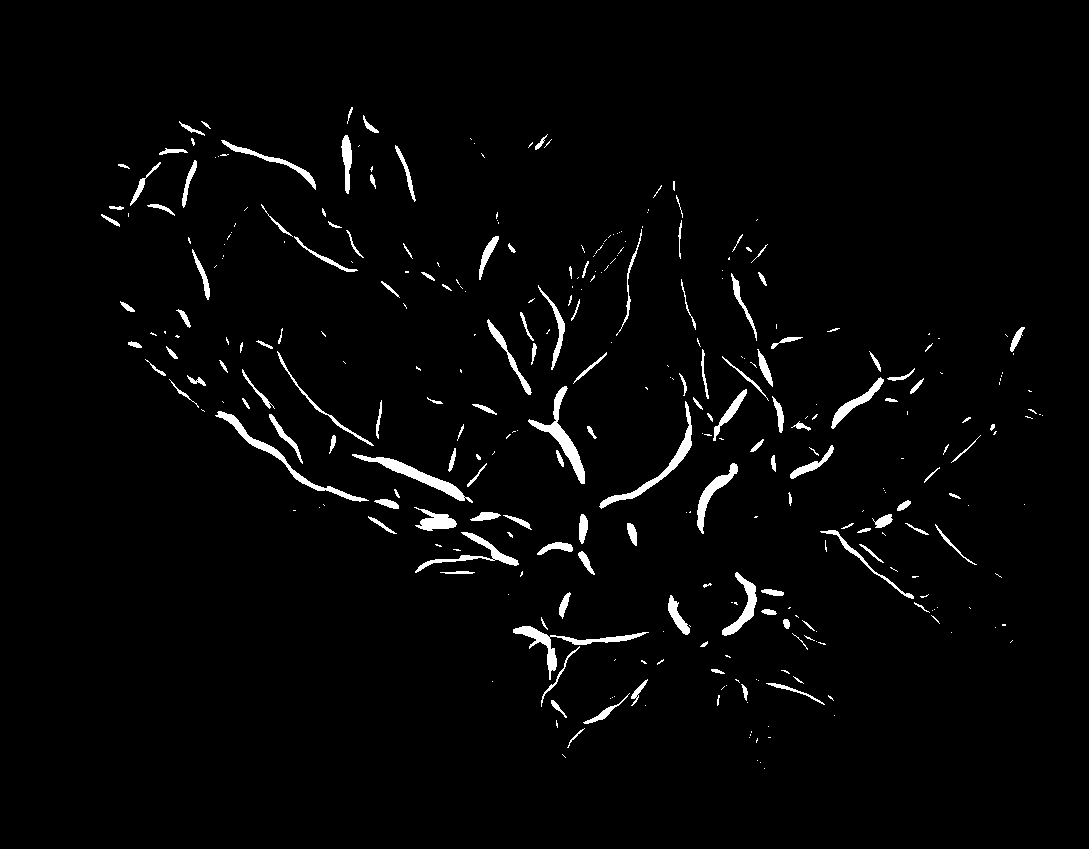
\includegraphics[width=0.48\linewidth]{qthresh_demo_q95}}
	\subfloat[scalewise percentile filtering ($p=98$)]{
		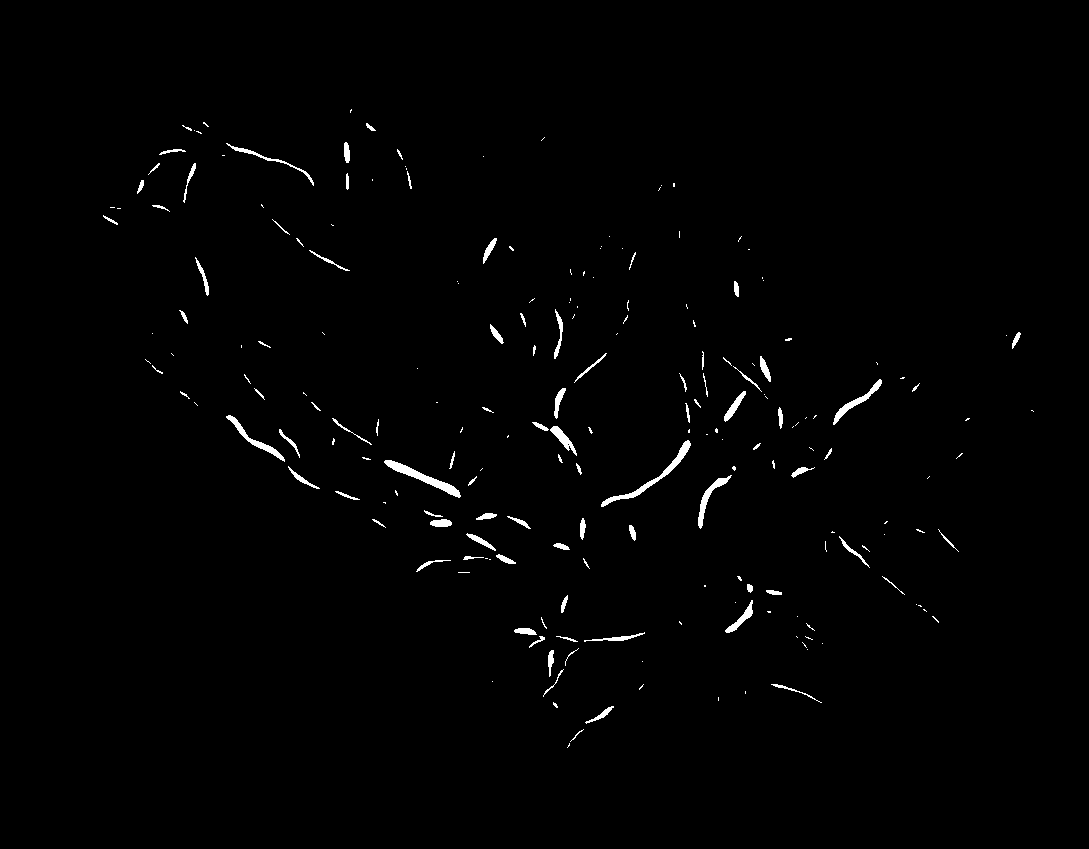
\includegraphics[width=0.48\linewidth]{qthresh_demo_q98}} \\
	\caption{Nonzero-percentile thresholding of \Vmax (95th and 98th percentile)}.
	\label{fig:qthresh_demo}
\end{figure}

Of course, the downside of this method is that we do not know in general the size of the network, and  we may miss entire branches of the vascular network if there is a large amount of curvilinear content elsewhere in the image that is simply less prominent than some other features which are prominent at the same scale. An additional caveat of this method is that, since all scales are given equal importance, this method could introduce a large amount of noise if the range of scales probled $\Sigma$, in particular the extremes $\sigma_{\min}$ and $\sigma_{\max}$ are not chosen carefully. That being said, the avantage of this method is that smaller scale features are more reliably extracted, whereas the slightly weaker Frangi signal at smaller scales causes smaller scale phenomena to less likely show up in a fixed threshold extraction.




%\subsection{Method D: Scale Based Sieving}
%
%Our final approach seeks to include not only pixels at each scale that pass a high threshold, but also adjacent pixels at that scale that pass a lower threshold. We proceed as follows. At each scale, take a low threshold, then label each connected region. Then, iterate through each labeled region and add to the final approximation any labeled region that contains a pixel that passes a higher threshold.

\subsection{Method C: Trough Filling}
As we discussed in \cref{sec:signed-frangi-filter}, we can simultaneously calculate the Frangi filter for light and dark curvilinear structures without any added computation time. We shown the signed result of the  Frangi filter at different scales two examples in \cref{fig:signsweep-1} and \cref{fig:signsweep-2}, we can simultaneously calculate calculate the Frangi filter response for bright curvilinear features (dark background) and dark curvilinear features (dark background). These two figures are the analogues to \cref{fig:scalesweep-1} and \cref{fig:scalesweep-2}. Since the Frangi filter normally throws away any response where $\lambda_2 < 0$ (if dark curvilinear features are targeted) or $\lambda_2 >0$ (if light curvilinear features are targeted), we lose no computation time at all by simply keeping both, although we must store more results. After computing the multiscale result, we can easily separate these into a positive and a negative strain, which we will denote $\VSigmapos$ and $\VSigmaneg$, and then merge each as we would with a traditional multiscale Frangi filter, giving us
\Vmaxpos and \Vmaxneg. That is, our \Vmaxpos is the same as our \Vmax in a conventional Frangi filter, and \Vmaxneg is the same result as if we had taken the Frangi filter while only looking for the opposite type (light/dark) curvilinear feature. Plotting $\Vmax$ over a scale of $[-1,1]$ demonstrates an interesting effect. Whereas the Frangi filter generally is not reliable in terms of accurately predicting widths, we \textit{can} get a sense of the width by looking at where there is a relatively strong response of opposite sign.

\begin{figure}[p] \centering
  \subfloat{		\label{fig:signsweep-1p}\includegraphics[width=\linewidth]{{{signsweep_stitch_BN2315363_plate}}}
  } \\[-0.5cm]
  \subfloat{		\label{fig:signsweep-1i}\includegraphics[width=\linewidth]{{{signsweep_stitch_BN2315363_inset}}}
  } \\[-0.5cm]
  \subfloat{		
    \label{fig:signsweep-1c}\includegraphics[width=.75\linewidth]{{{signsweep_colorbar}}}
  } \\
  
  \caption{Signed Frangi output (plate and inset) (example 1)}
  \label{fig:signsweep-1}
\end{figure}

\begin{figure}[p] \centering
  \subfloat{		\label{fig:signsweep-2p}\includegraphics[width=\linewidth]{{{signsweep_stitch_BN5280796_plate}}}
  } \\[-0.5cm]
  \subfloat{		\label{fig:signsweep-2i}\includegraphics[width=\linewidth]{{{signsweep_stitch_BN5280796_inset}}}
  } \\[-0.5cm]
  \subfloat{		
    \label{fig:signsweep-2c}\includegraphics[width=.75\linewidth]{{{signsweep_colorbar}}}
  } \\
  \caption{Signed Frangi output (plate and inset) (example 2)}
  \label{fig:signsweep-2}
\end{figure}
That is, at the "foot" of every trough on either side, we can see a bordering curvilinear structure of opposite sign. We perform strict Frangi filtering and separate the positive and negative components. We then perform a different threshold for each signed portion of the Frangi response--a strict one (say $\alphapos > .3$) for the conventional $\Vmax$, and a much looser one for our opposite signed $\Vmaxneg > \alphaneg = .01$. We also truncate the scales we consider for calculating $\Vmax^{(-)}$, considering only the 6 smallest scales of 20, since we empirically notice that the bordering curvilinear features are consistently narrower than the vessels themselves.

We will refer to any pixel where $\Vmaxpos > \alphapos$ as ``in the trough'' (assuming dark curvilinear features), and any pixel where $\Vmaxneg > \alphaneg$ as potentially ``on the lip'' of the trough. The process of ``trough-filling'' then proceeds as follows.  For each pixel within the trough, we iterate over disks of integer radius and dilate the pixel by a disk of that radius if that disk includes a point on the lip, where $\Vmaxneg > \alphaneg$. This allows us to extend the Frangi output from the point where it's strongest all the way to the base of the curvilinear structure, providing a much better indication of the true width of the curvilinear structure.

\begin{figure}[p] \centering
  \subfloat{		\includegraphics[width=\textwidth]{{{fig-insetBN0164923}}}
  } \\[-0.5cm]
  \subfloat{		
    \includegraphics[width=\textwidth]{{{fig-BN0164923}}}
  } \\
  \caption{Trough dilation process (inset and plate)}
  \label{fig:trough_dilation}
\end{figure}

In \cref{fig:trough_dilation} we demonstrate the process of creating a trough dilation segments. The top left is the original sample. This was a $N=20$ Frangi filter with log range from -1.5 to 3.2 and Frangi parameters $\beta=0.15$ and $\gamma=1.0$ The middle top and top right shows $\Vmax^{(+)}$ and $\Vmax^{(-)}$ respectively. The bottom then shows the two markers 
 $\Vmax^{(-)} > \alpha^{(-)} = 0.01$ (in red) and
 $\Vmax^{(+)} > \alpha^{(-)} = .3$ (in blue). We build $\Vmax^{(-)}$ only using the 6 smallest scales, since the lighter curvilinear 'lip' of the trough is of smaller radius than the radius of the trough itself. Probing at too large scales could perhaps introduce noise. We will call this subset $\Sigmaneg \subset \Sigma $ and choose $\Sigmaneg=\{\sigma_1 , ... , \sigma_6\}$.
 
 

\section{Nonfrangi Segmentation Methods}

Of course, there are many other viable methods of segmentation. We refer to \autocite{anghel2018placental} for several high-performing (albeit considerably resource intensive) segmentation methods on this dataset, namely involving shearlets, Laplacian eigenmaps, and a conditional generative adversarial network.

We will be content in the present paper to simply compare our results to a relatively fast technique that is not based on differential geometry or morphology, but instead that of a global threshold on the grayscale image. Although many viable thresholding algorithms exist, we opt for an intermeans threshold, or the Ridler-Calvert or ISODATA method, as described in \autocite{isodata}, which is implemented in \textrm{scikit-image} as \textrm{filters.threshold\_isodata}. This functions uses an iterative process to find the smallest threshold which is midway between the mean intensities of the high pixels and the low pixels. In other words, the optimal $\alpha_{\textrm{ISO}}$ satisfies

\begin{equation} \label{eq:ISODATA}
\alpha_{\textrm{ISO}} = \arg\min_{\alpha} \left( \frac{1}{2} \Big[
\textrm{mean}\left\{ \img(x,y) \;|\; \img(x,y) \le \alpha \right\} 
+
\textrm{mean}\left\{ \img(x,y) \;|\; \img(x,y) >   \alpha \right\}
 \Big]
 \right)
\end{equation}

Since the vascular structure in our image domain is darker than the background, we select pixels
where $\img(x,y) < \alphaiso$.



\section{Comparison of Segmentation Methods}
In our demonstration of segmentation methods across all 201 samples in our image domain, we use the preprocessing procedure described in \cref{ch:research-protocol}.

Our multiscale Frangi filter setup involves 20 scales spaced logarithmically from $\sigma_1 = 2^{-1.5} \approx .35$ to $\sigma_{20} = 2^{3.2} \approx 9.20$. We will compare the results of 6 different segmentation methods using three different parametrizations of the Frangi filter. These parametrizations and segmentation methods with specific parameter choices are summarized in \cref{tab:segmentation-methods,tab:segmentation-parametrizations}.


\begin{table}[h]
  \caption{Summary of Segmentation Methods}
\centering
\begin{tabular}{|c|l|p{4.5cm}|}
  \hline
  Label & Description & Parameter(s) \\ \hline
  thresh-high & Fixed threshold of Frangi filter $\Vmax > \alpha $ & $\alpha = 0.3$ \\ \hline
  thresh-low &  Fixed threshold of Frangi filter $\Vmax > \alpha $ & $\alpha = 0.2$ \\ \hline
  snz-p-high & scalewise nonzero percentile filtering of \VSigma & $q = 95$ \\ \hline
  snz-p-low & scalewise nonzero percentile filtering of \VSigma & $q = 98$ \\ \hline
  TF & trough-filling method &
    \parbox{4.5cm}{$\alphapos=0.3,\;\alphaneg=.01,\\
                    \Sigmaneg=\{\sigma_1,\cdots,\sigma_6\}$} \\ \hline
  ISODATA & Non-Frangi global threshold & see \cref{eq:ISODATA} \\ \hline
\end{tabular}

\label{tab:segmentation-methods}
\end{table}

\begin{table}[h]
  \caption{Summary of Frangi Parametrizations for Segmentation Demo} 
  \centering
  \begin{tabular}{|c|c|c|}
    \hline
    Label  & $\beta$ & $\gamma$ \\ \hline
    standard & $0.5$ & $0.5$ \\ \hline
    semistrict & $0.15$ & $0.5$ \\ \hline
    strict & $0.15$ & $1.0$ \\ \hline
  \end{tabular}

\label{tab:segmentation-parametrizations}
\end{table}


In \cref{fig:seg-montage-example}, we look at the results of our various segmentation procedures for a typical well behaved sample. We can see that there are fewer false negatives for strict parametrization than with a standard parametrization. Even though the best MCC score across the 10 demonstrated in \cref{fig:seg-montage-example} is achieved by trough filling under standard parametrization, we note that trough filling in the strict parametrization has comparatively fewer false negatives and much higher precision. The highest precision is achieved by our higher fixed threshold. Thus, we should see the high MCC score achieved by the trough filling method as a testament to the usability of a simpler threshold (such as FT-high) as a precursor to more complete segmentation methods.


In \cref{fig:scoring-boxplots} we graph the MCC and precision scores across our entire set of 201 images. In each boxplot, the median is labeled, with first and third quartiles making up the edges of the box. The ends of the whiskers represent  $median \pm 1.5*(Q3-Q1)$. The quantity ($Q3-Q1$), the difference of the third quartile (where $p=75$) and first quartile (where $p=25$) is the so-called interquartile range \autocite{scipy}. Outliers outside of those whiskers, from samples such as those in \cref{fig:bad-gallery}, are plotted as individual data points.

Across all samples, maximum precision was achieved by the higher fixed threshold of $\alpha =0.3 $ in all but 22 samples, and the trough filling method offered the best MCC in about three-fourths of the samples (51 of 201). Where the trough filling method was not most accurate, we noticed that the $q=95 $ nz-percentile method had a slightly higher MCC score. From viewing the samples, we see that noise from the umbillical cord insertion point still hinders a number of samples, causing noise within the Frangi filter. 

From viewing \cref{fig:scoring-boxplots} we can see that, for any of the
three parametrizations, we achieve a higher precision and lower MCC from increasing the fixed threshold. The same trend occurs between scalewise nz-p segmentations when we increase the quartile (from q=95 to q=98). The median MCC of the ISODATA method was lower than all Frangi-based segmentations across all with the exception of the highest fixed threshold under strict parametrization--although the latter method has the highest median precision score by far. ISODATA has a much lower precision than any of the other methods present here.

We notice a larger number of MCC outliers for scalewise methods than fixed threshold based methods. We theorize that this is due to the difficulty in knowing \textit{a apriori} an appropriate range of scales to probe. Future work therefore could immediately improve upon the results of this chapter by finding an appropriate range or, more likely, a normalization factor for scales that makes the success of segmenation less dependent on $\sigma_{min}$ and $\sigma_{max}$.

From \cref{fig:scoring-boxplots} we also notice that the MCC and precision for each scalewise method is not as affected by changes in parameterization as the fixed methods. We suggest that is because stricter parameters have the effect of rescaling to some degree within each step of the multiscale method, so that the same pixels at each scale ultimately occur at each scale's highest percentiles.

Looking at \cref{fig:seg-montage-example2}, we see a situation in which scalewise methods do poorly. The $p=95$ scalewise method under either parametrization, as well as the lower fixed threshold under standard parametrization show some curvilinear noise between vessels. These come from larger scales, so there is apparently no signficant vasculature being picked up at the largest scales, causing noise to appear. This is less pronounced for fixed thresholding using stricter parameters, although some of this noise can still be seen in the strict Frangi's \Vmax plot.


\begin{figure}[p] \centering
  \subfloat[standard parametrization]{ 	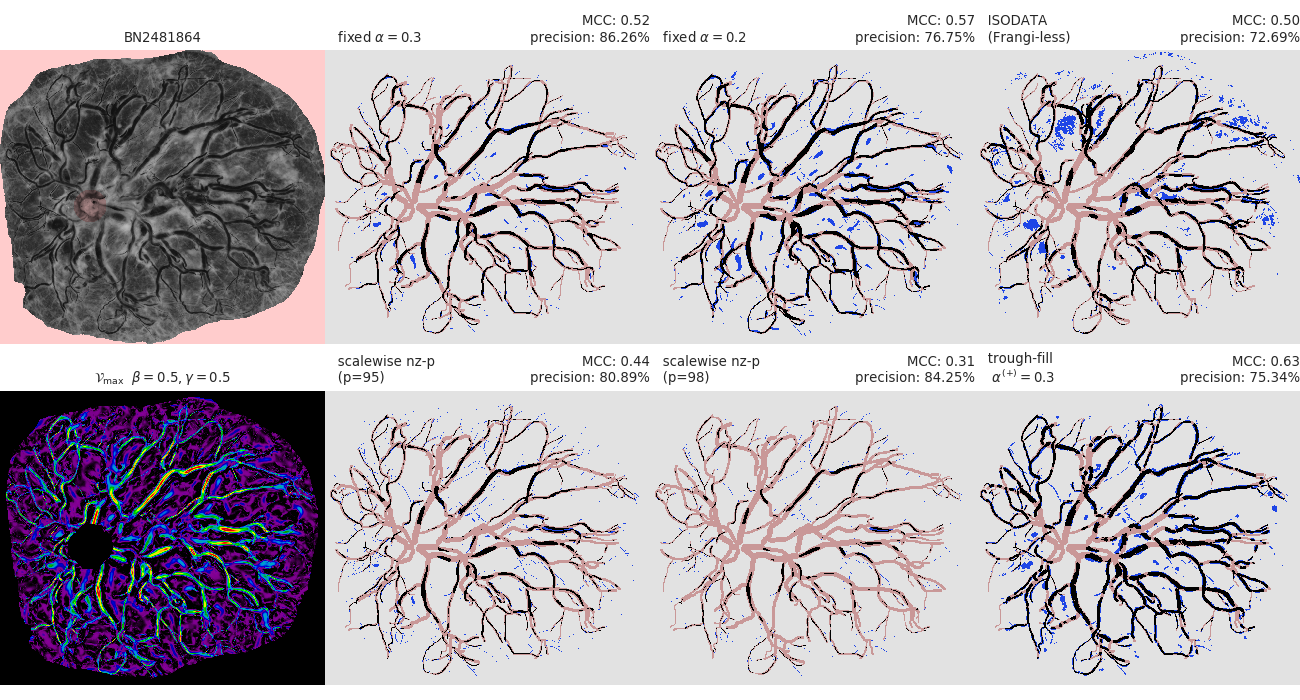
\includegraphics[width=\textwidth]{fig-BN2481864-standard-seg}} \\
  \subfloat[strict parametrization]{ 	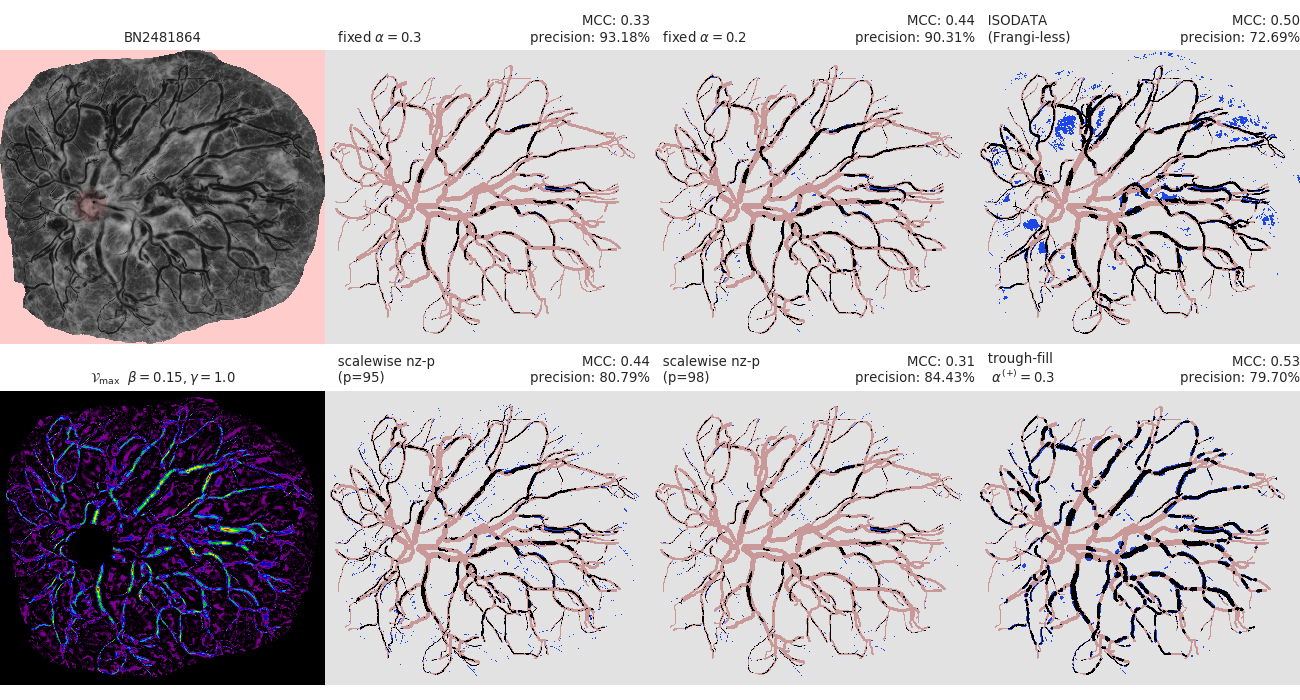
\includegraphics[width=\textwidth]{fig-BN2481864-strict-seg} }
  \caption{Segmentation results, example 1 (standard and strict parametrization)}
	\label{fig:seg-montage-example}
\end{figure}

\begin{figure}[p] \centering
	\subfloat[standard parametrization]{ 	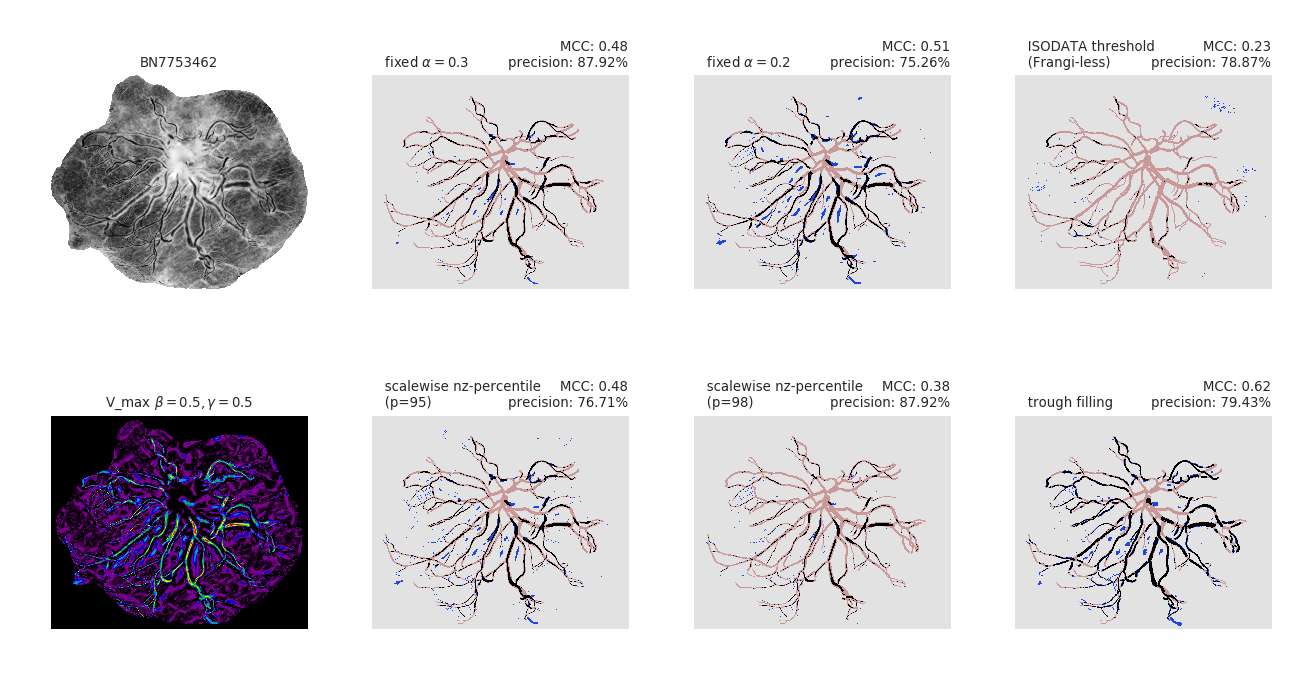
\includegraphics[width=\textwidth]{fig-BN7753462-standard-seg}} \\[-0.5cm]
%    \subfloat{ 	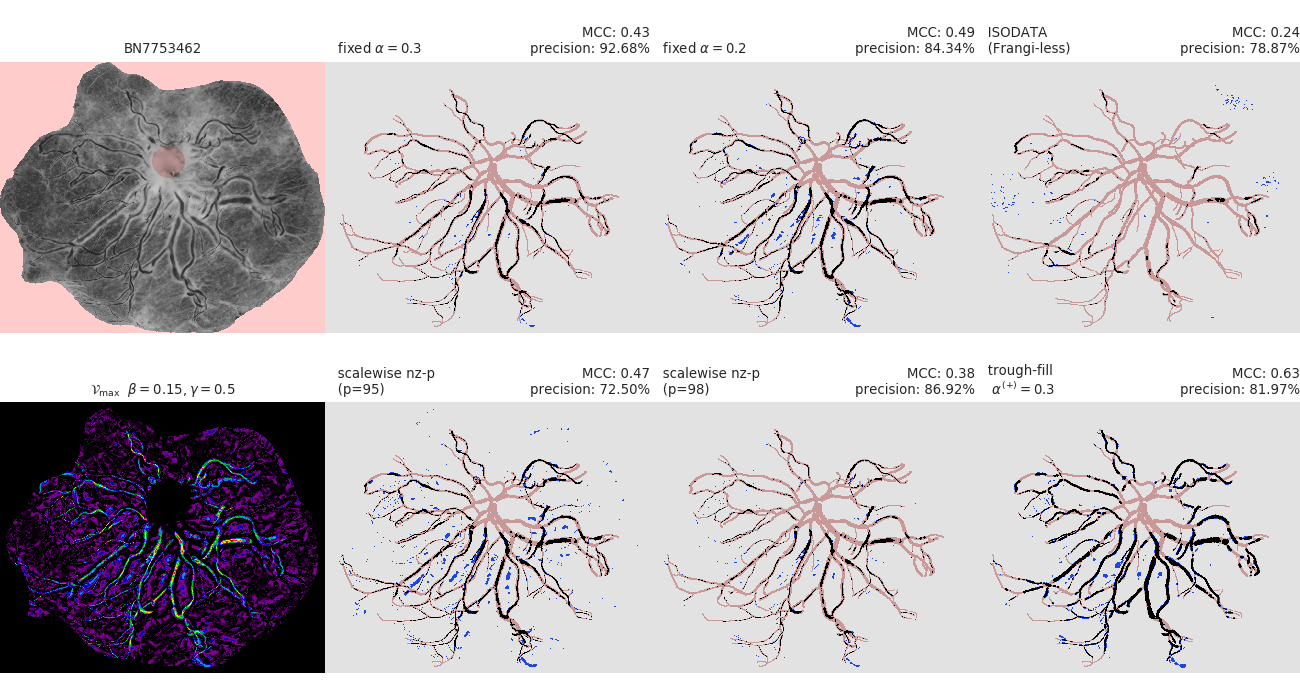
\includegraphics[width=\textwidth]{fig-BN7753462-semistrict-seg} } \\[-.5cm]
	\subfloat[strict parametrization]{	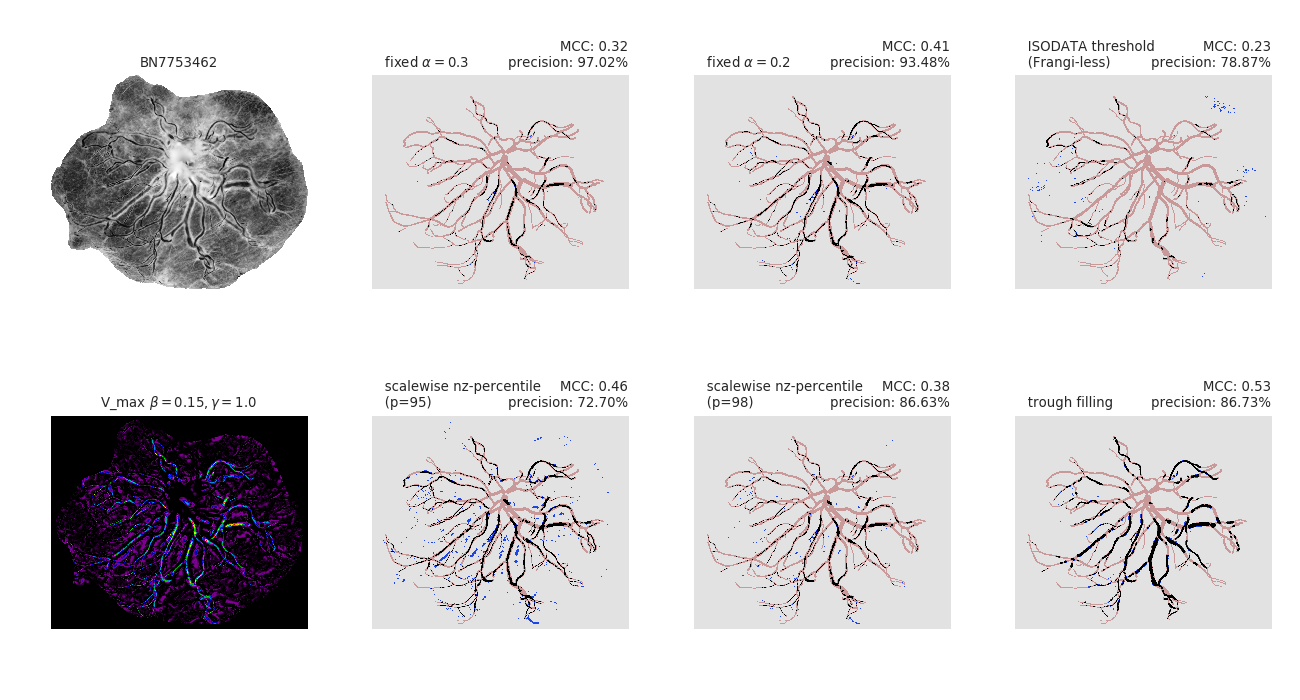
\includegraphics[width=\textwidth]{fig-BN7753462-strict-seg} }
	\caption{Segmentation results, example 2 (standard and strict parametrization)}
	\label{fig:seg-montage-example2}
\end{figure}

\begin{figure}[p] \centering
  \subfloat[standard Frangi parametrization ($\beta=0.5, \gamma=0.5$)]{  
            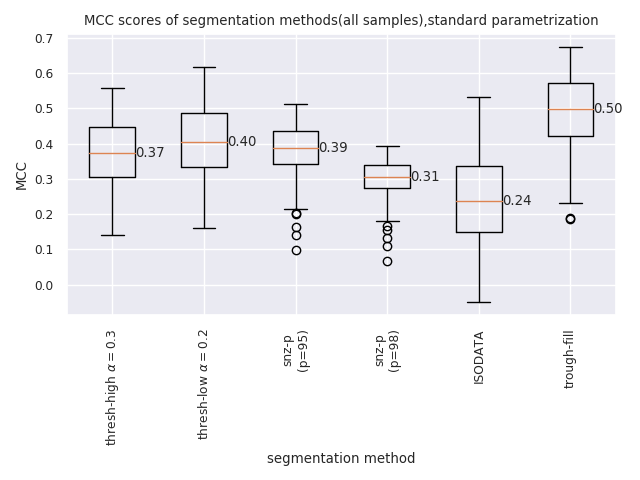
\includegraphics[width=0.5\textwidth]{all-MCC-boxplot-standard} 
            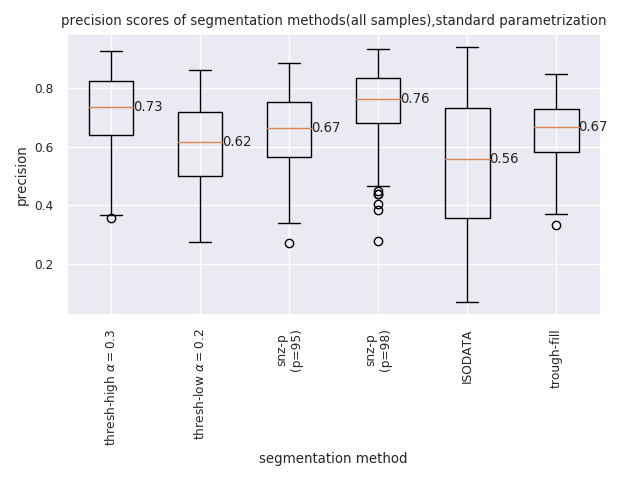
\includegraphics[width=0.5\textwidth]{all-precision-boxplot-standard} } \\
  \subfloat[semistrict Frangi parametrization ($\beta=0.15, \gamma=0.5$)]{ 
            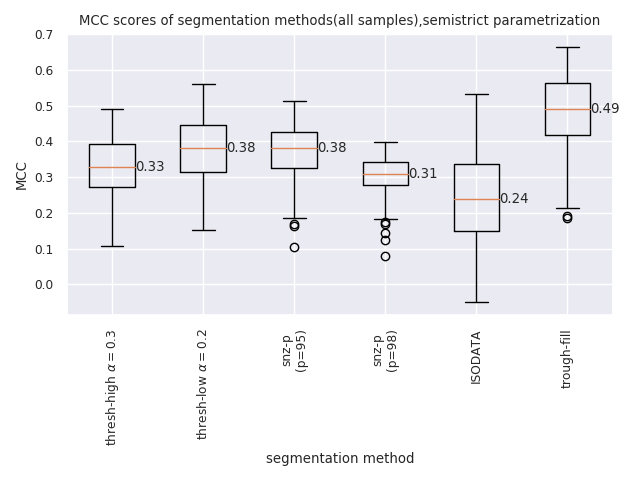
\includegraphics[width=0.5\textwidth]{all-MCC-boxplot-semistrict} 
            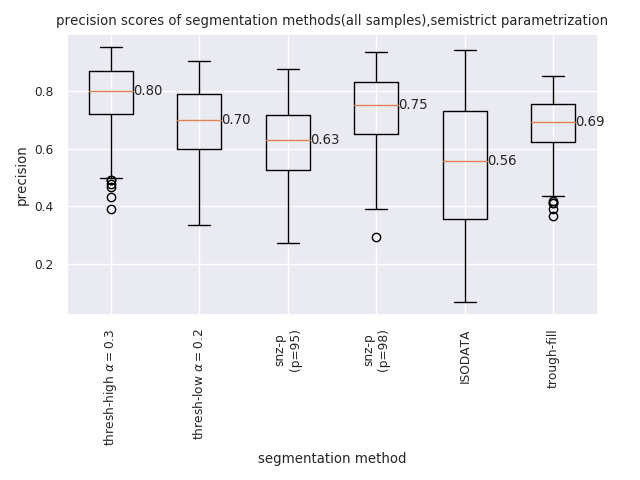
\includegraphics[width=0.5\textwidth]{all-precision-boxplot-semistrict} } \\
  \subfloat[strict Frangi parametrization ($\beta=0.15, \gamma=1.0$)]{ 
            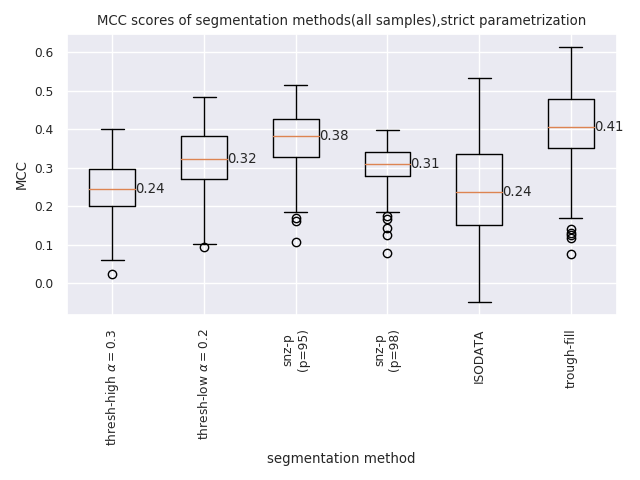
\includegraphics[width=0.5\textwidth]{all-MCC-boxplot-strict} 
            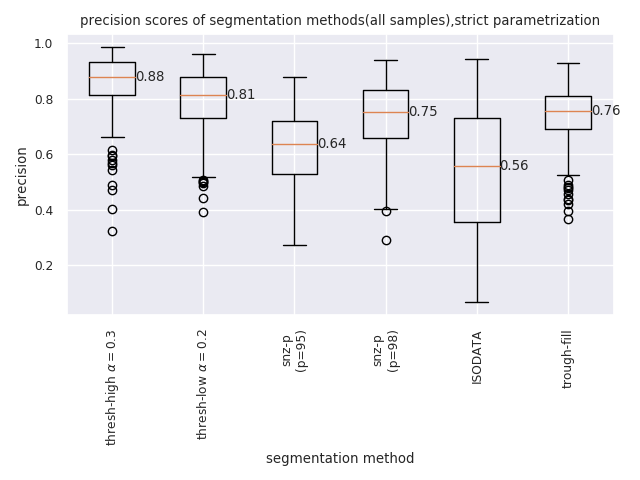
\includegraphics[width=0.5\textwidth]{all-precision-boxplot-strict} } \\
      \caption{MCC and precision of segmentation methods (201 samples)}
      \label{fig:scoring-boxplots}
\end{figure}

%\section{Scale-wise Random Walker: A demo}
%
%
%We observed that areas where Frangi scores are zero in well-behaved samples seem to neatly outline prominent vascular features. Following this idea, we employed a random walker segmentation \autocite{Grady-Random-Walks} (which is implemented by \texttt{scikit-image}). Random walk segmentation comes about by solving a diffusion problem over a discrete array (in this case, the Frangi vesselness score itself) given starting markers. At each scale, we positively labeled pixels whose Frangi score was very high ($\Vsigma(x_0,y_0) > .4$), and negatively labeled pixels whose score was $0$ (i.e. where the leading principal eigenvalue was positive). The result of this technique is demonstrated in \cref{fig:rw-demo-scalewise} and the result (along with the original sample for comparison) is shown in \cref{fig:rw-demo-merged}.
%In \cref{fig:rw-demo-scalewise}, the first column is the Frangi vesselness score at that scale, where black is a score of 0, to emphasize the difference between a score of zero and even a very small positive score, which appear in blue. The middle score are markers passed to the random walker--blue are seeds labelled with a ``1'' (where the Frangi vesselness score is 0), green is labeled ``2'' (where \Vmax > .4), and purple represents unknowns that will either assigned either label. In the last column, the result of the random walker is given--areas that have been added to the label ``2'' are shown in yellow. Although the result of random walker segmentation is technically a binary matrix, we still show the original seeds of label 2 in green for easier comparison. Similarly, the purple in the right column has actually been labeled ``1'' for non-vascular, but is left in its original color to emphasize what was assigned background. In \cref{fig:rw-demo-merged} we show the original image and the result of merging all positively marked pixels at each scale. Black means the pixel was unmatched, while increasing colors of blue (larger scales) to white (smaller scales) indicate the smallest scale from which a pixel was marked after the random walker technique. \vtodo{Do I need to over this in math methods section?} Though we shall set up the multiscale method slightly differently in \cref{ch:results-analysis}, we used a Frangi anisotropy coefficient of $\beta=0.35$ , and 12 scales logarithmically spaced from $\sigma_1 = 2^{-1.5} $ to $\sigma_{12} = 2^{3.5}$ to generate these figures. There is a parameter for the random walker algorithm (unfortunately also called $\beta$) which serves as a diffusion penalization coefficient (larger values making diffusion over the image less likely). We used \texttt{scikit-image}'s default value of 130. 
%
%\begin{figure}[p] \centering
%  \subfloat{
%    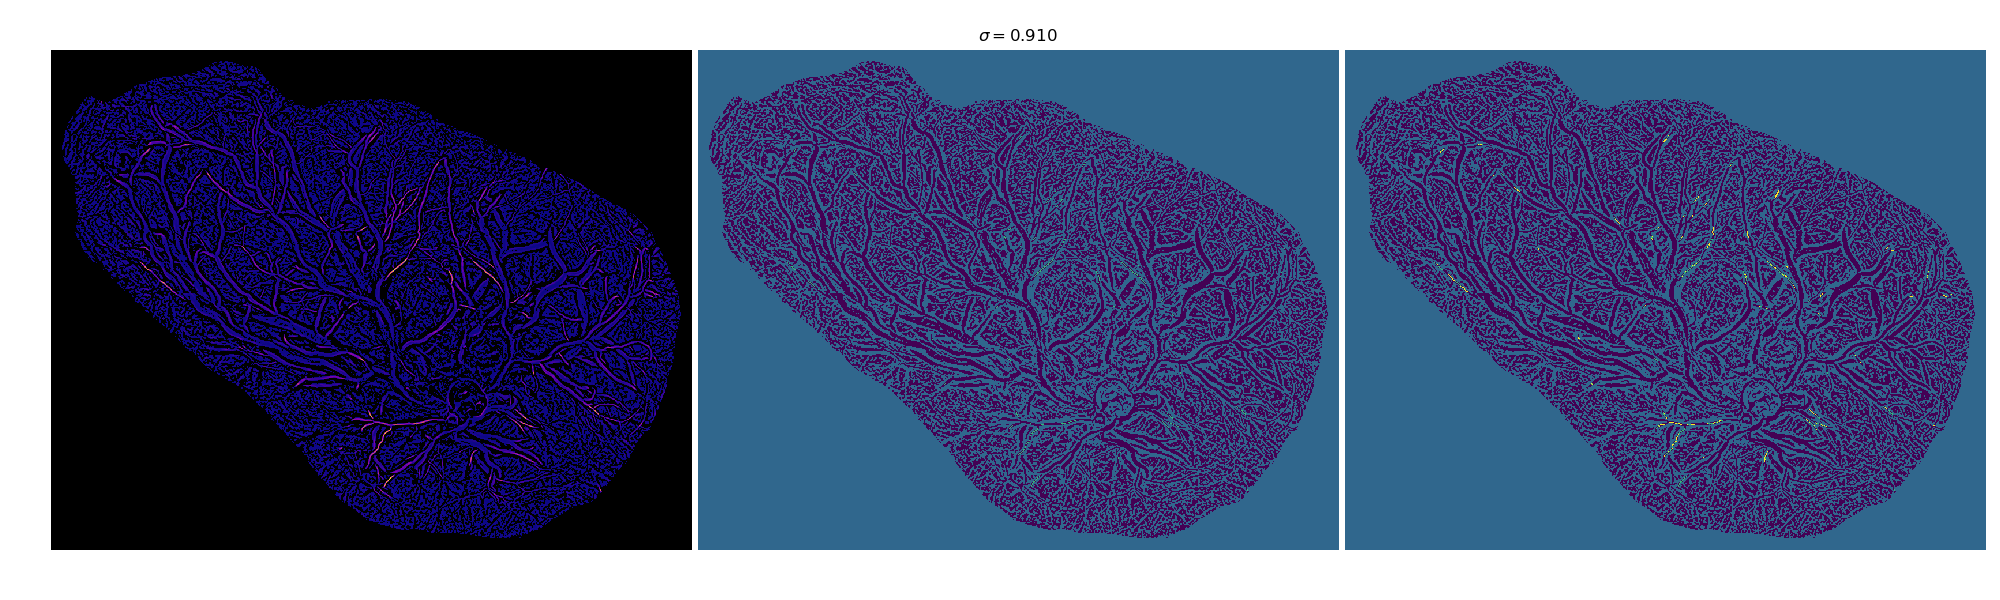
\includegraphics[width=\textwidth]{rw_demo_scale_03}
%  }\\[-0.5cm]
%  \subfloat{
%    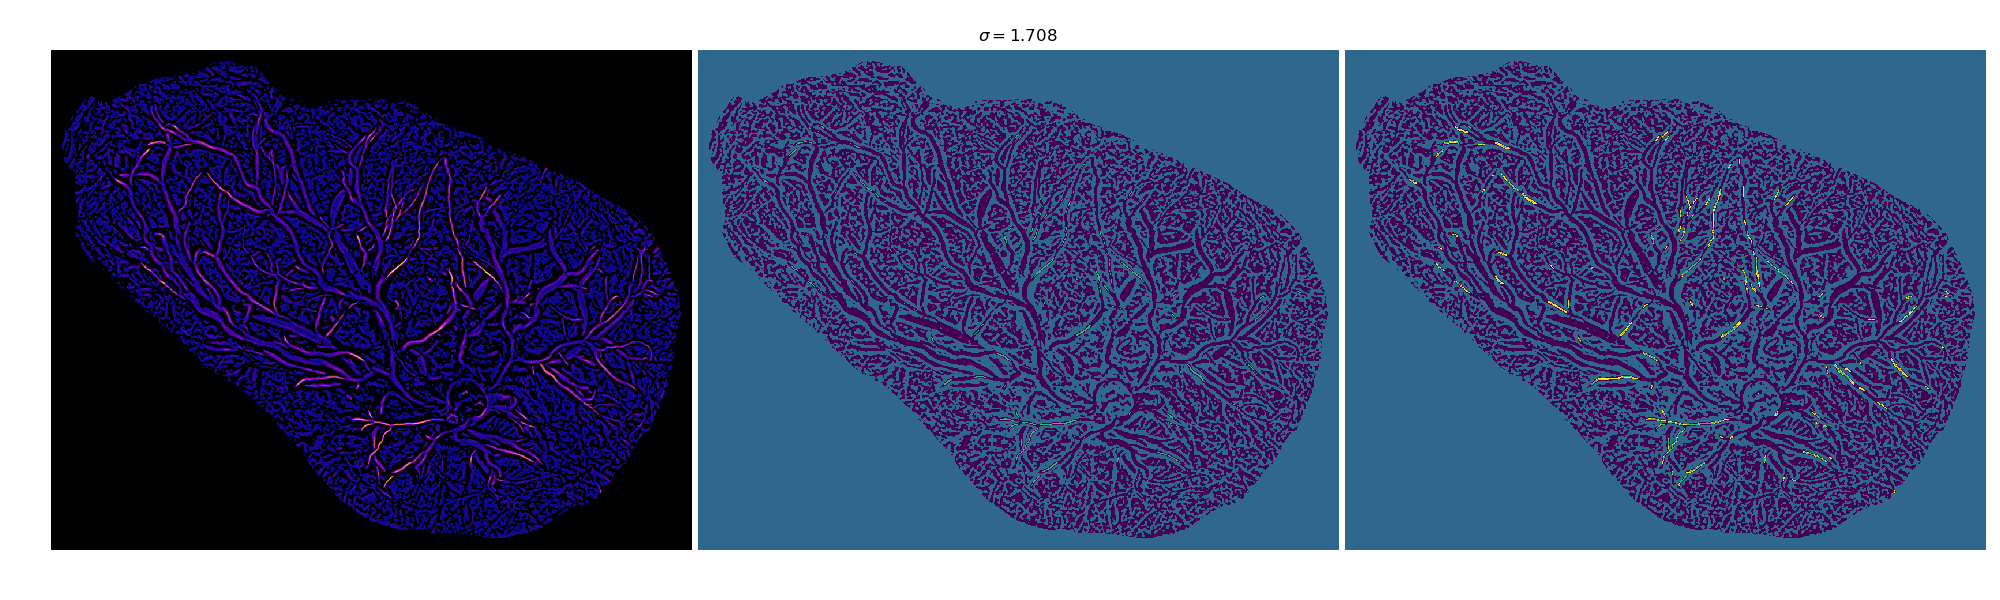
\includegraphics[width=\textwidth]{rw_demo_scale_05}
%  }\\[-0.5cm]
%  \subfloat{
%    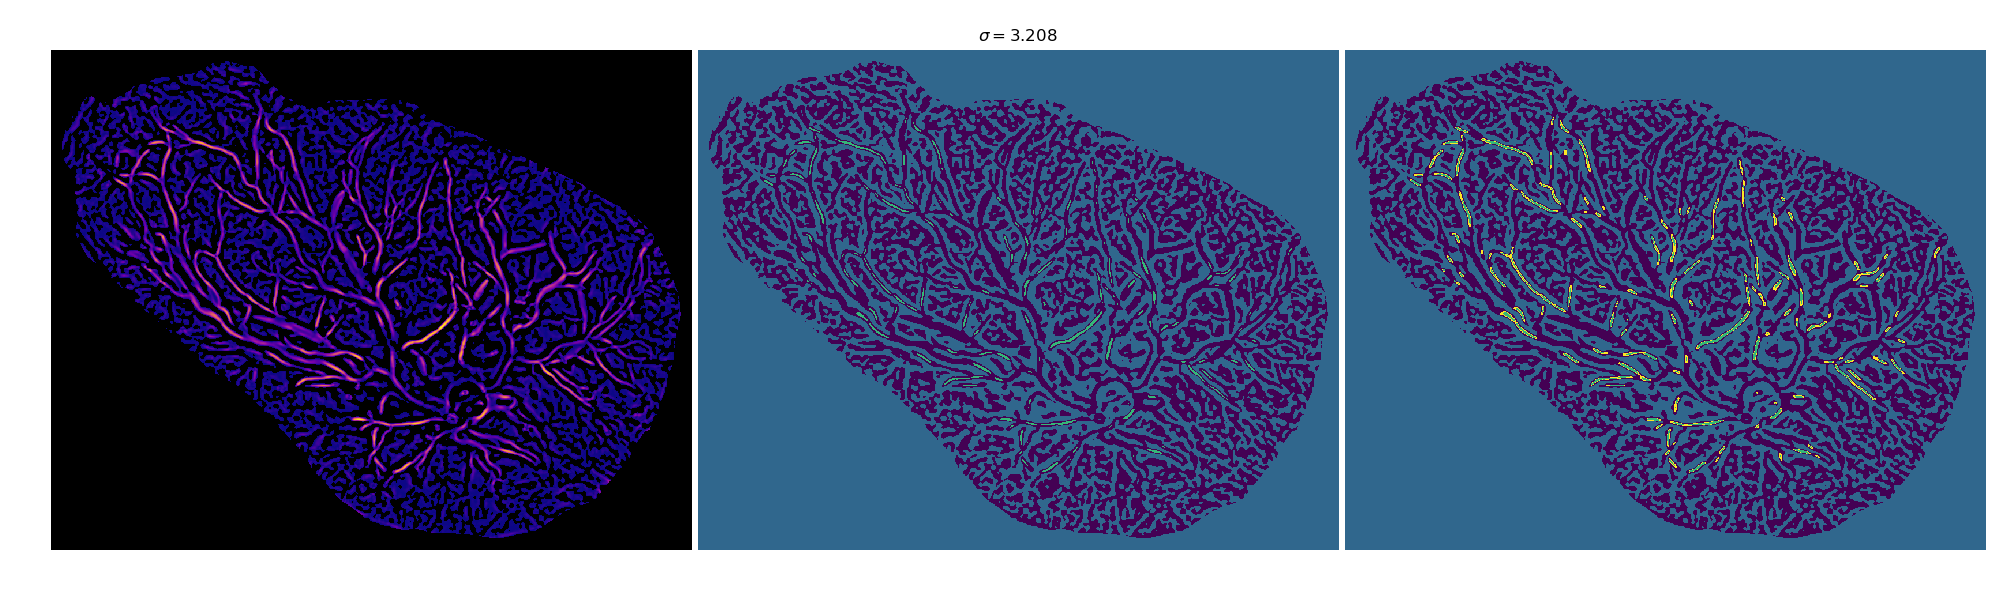
\includegraphics[width=\textwidth]{rw_demo_scale_07}
%  }\\[-0.5cm]
%  \subfloat{
%    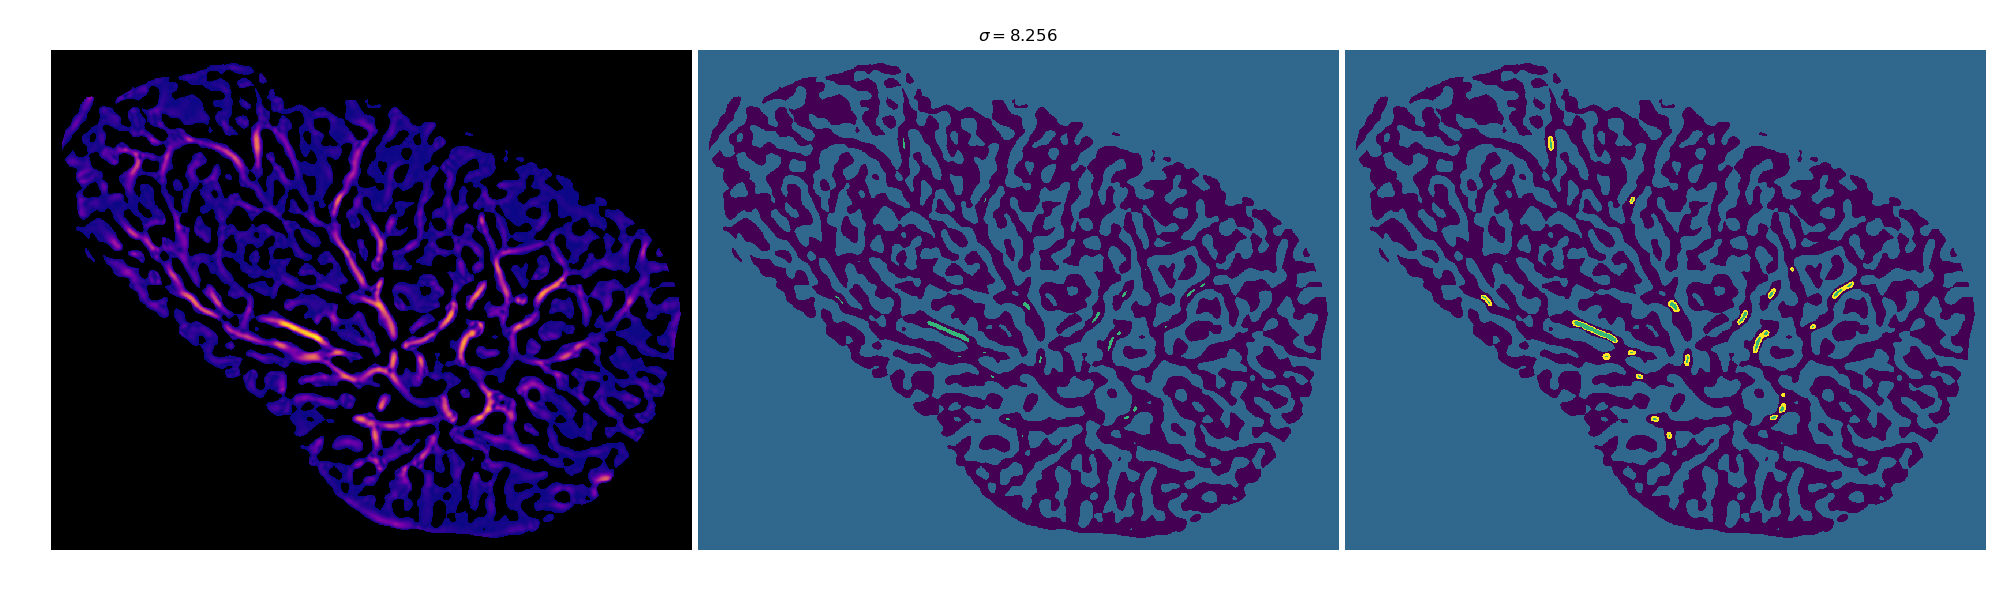
\includegraphics[width=\textwidth]{rw_demo_scale_10}
%  }
%  \caption{Scale-wise random walker segmentation (select scales)}
%  \label{fig:rw-demo-scalewise}
%\end{figure}
%
%
%\begin{figure}[t] \centering
%  \subfloat{
%    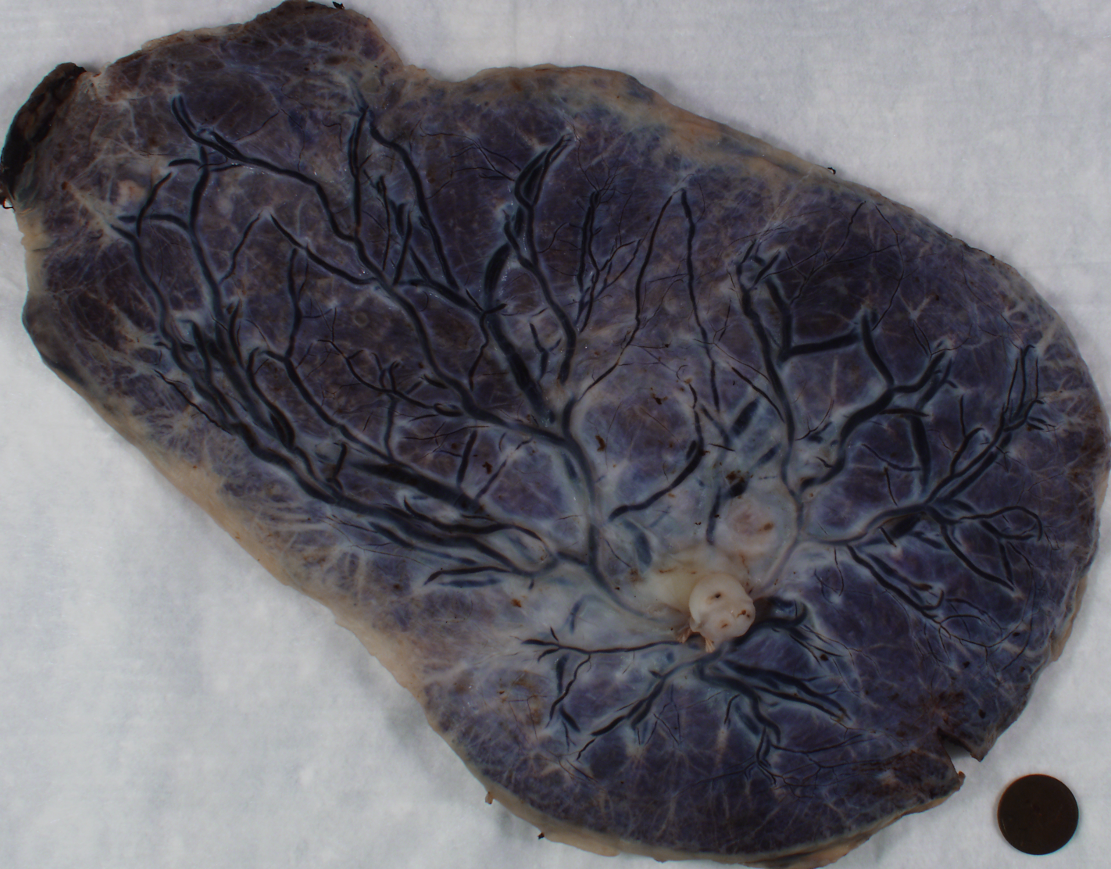
\includegraphics[height=0.4\textwidth]{rw_demo_base}
%  }
%  \subfloat{
%    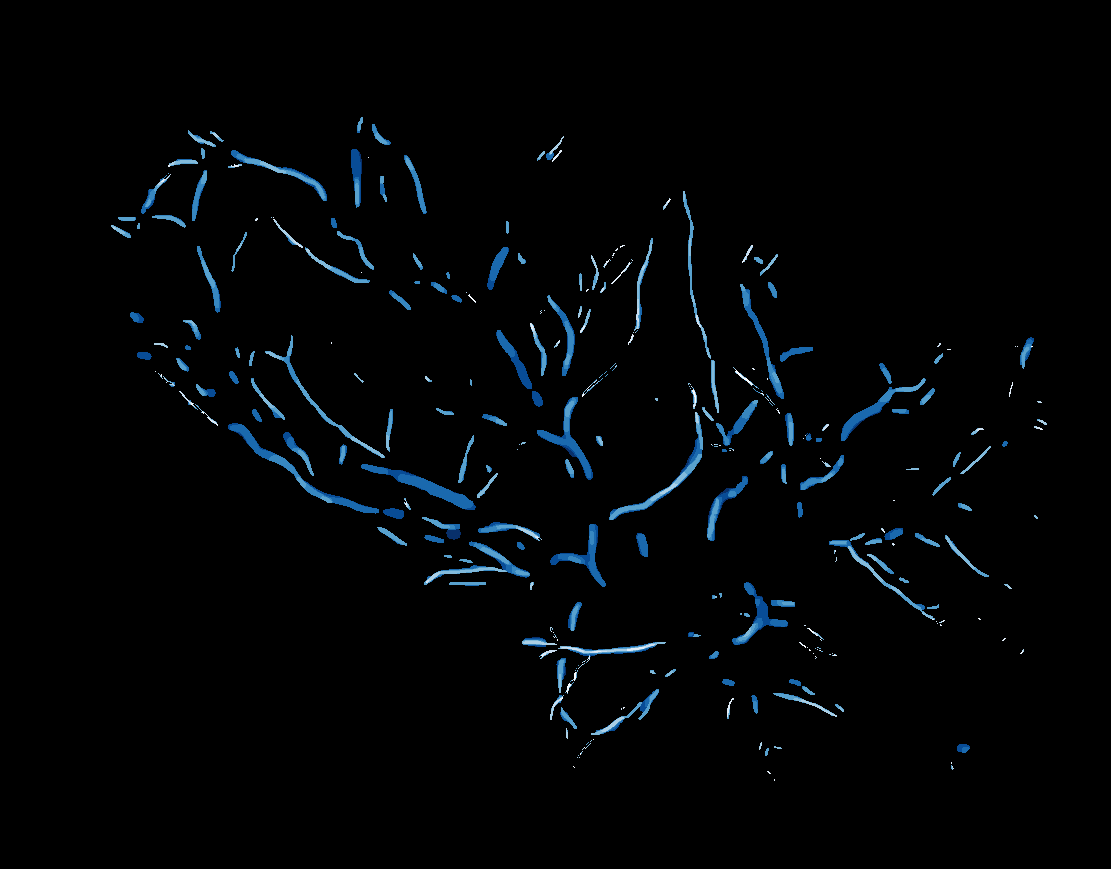
\includegraphics[height=0.4\textwidth]{rw_demo_labels}
%  }
%  \caption{Random walker segmentation (sample and merged result)}
%  \label{fig:rw-demo-merged}
%\end{figure}
\section{Network Completion} \label{sec:network-completion}
We can see from looking at the \Vmax outputs of our samples that even where gaps exist in the segmentation output, there is still \textit{some} Frangi output where the gap exists. For various reasons, the output might not be as strong at that particular region, but we can use that fact to bridge some of these gaps. To do so would be to achieve ``simple gap completion''--that is, connecting the vascular network to compensate for the shortcomings of a particular segmentation method. We differentiate this from ``predictive gap completion,'' which we will use to signify the problem of connecting the vascular network where the tracer themselves had to guess what was happening with the network. For example, the entire area surrounding the umbilical cord insertion point in \cref{fig:seg-montage-example2} is difficult to make out. The tracer ultimately used some knowledge of vascular network growth to predict what was happening in this region to produce the ground truth. Predictive gap completion would also need to be used to solve crossings of veins and arteries.

First, once we've produced a segmentation, we use morphological thinning to reduce it to one pixel width with \autocite{thinning} and look for endpoints of an otherwise connected point. Using a $3\times 3$ structuring element, we iterate over each pixel and identify how many local neighbors it has. If a pixel has zero or one local neigbors, we identify it as an endpoint of the partial network. After identifying these endpoints, we assign each a label $(i,j)$ depending on where the neighboring pixel is located, as according to \cref{fig:endpoint_labels}. We deem two endpoints potentially connectible only if they're not connected on the same side. That is, their labels $(i,j)$ and $(i',j')$ must have $i\ne i'$ or $j\ne j'$ (unless $i$ or $j$ is 1). For example, if an endpoint is connected to the partial network on its top side, any endpoint that connects to it cannot also be connected to a network on its top. If a pixel has no connections at all, with label $(1,1)$, we do not restrict its connetions at all. To save time (though we don't anticipate it will affect the result much), we also restrict pais from being more than a set distance away (in this case, 100 pixels in Euclidean length).

\begin{figure}
	\centering
	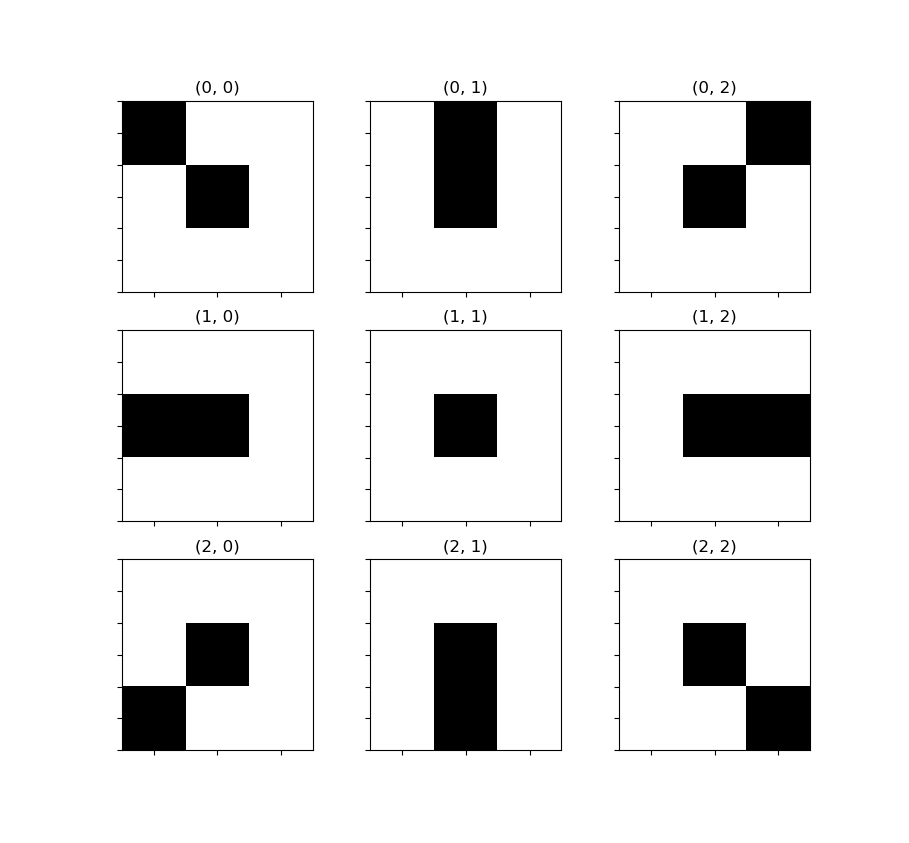
\includegraphics[width=.5\textwidth]{endpoint_labels}
	\caption{Endpoints labels based on adjacent neighbor location}
	\label{fig:endpoint_labels}
\end{figure}

After we limit the connections, we consider each pair of endpoints and draw a straight line segment between the two. If that passes through a point where $\Vmax$ is 0, we disallow that pair as well. We also disallow any line which crosses any part of the network which is known to exist.
\begin{figure}[p]
	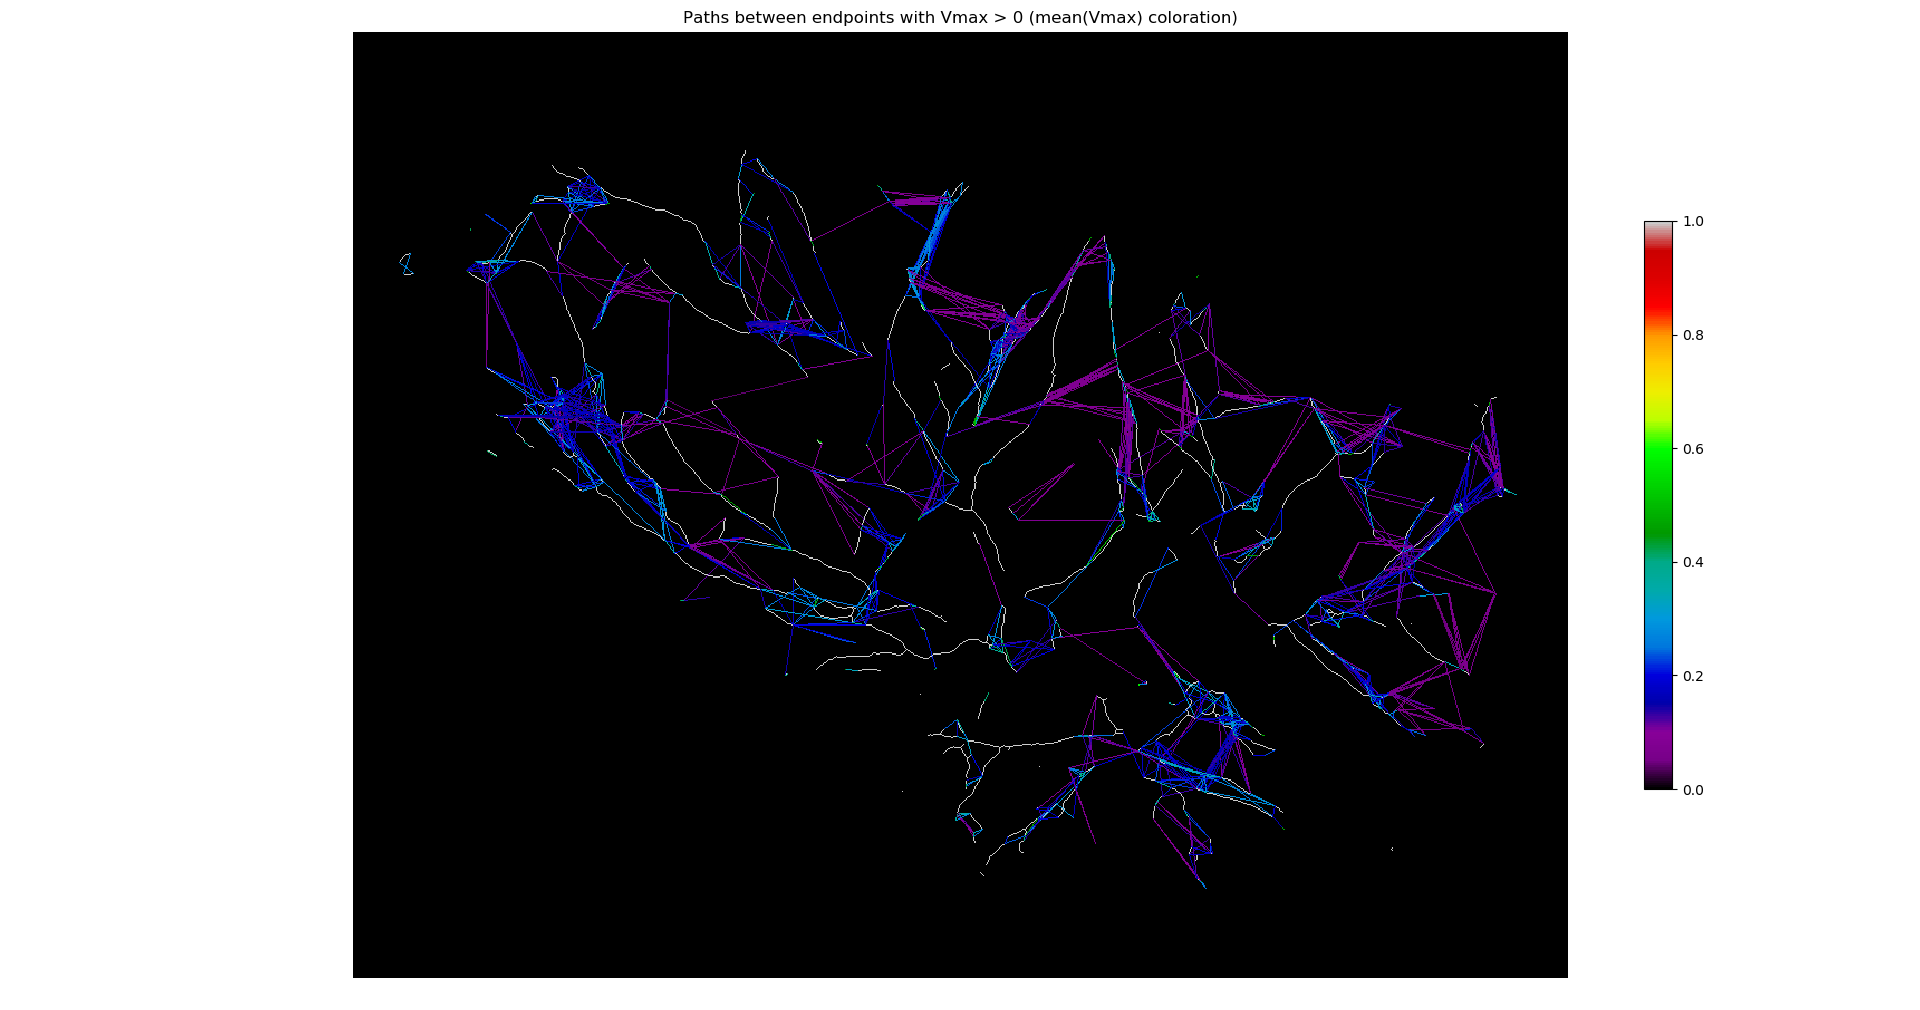
\includegraphics[height=0.4\textheight]{paths_between_endpoints_positive_score}
	\caption{All lines between endpoints with nonzero $\Vmax$}
	\label{fig:network-completion-connected-pairs}
\end{figure}
\begin{figure}[p] \centering
	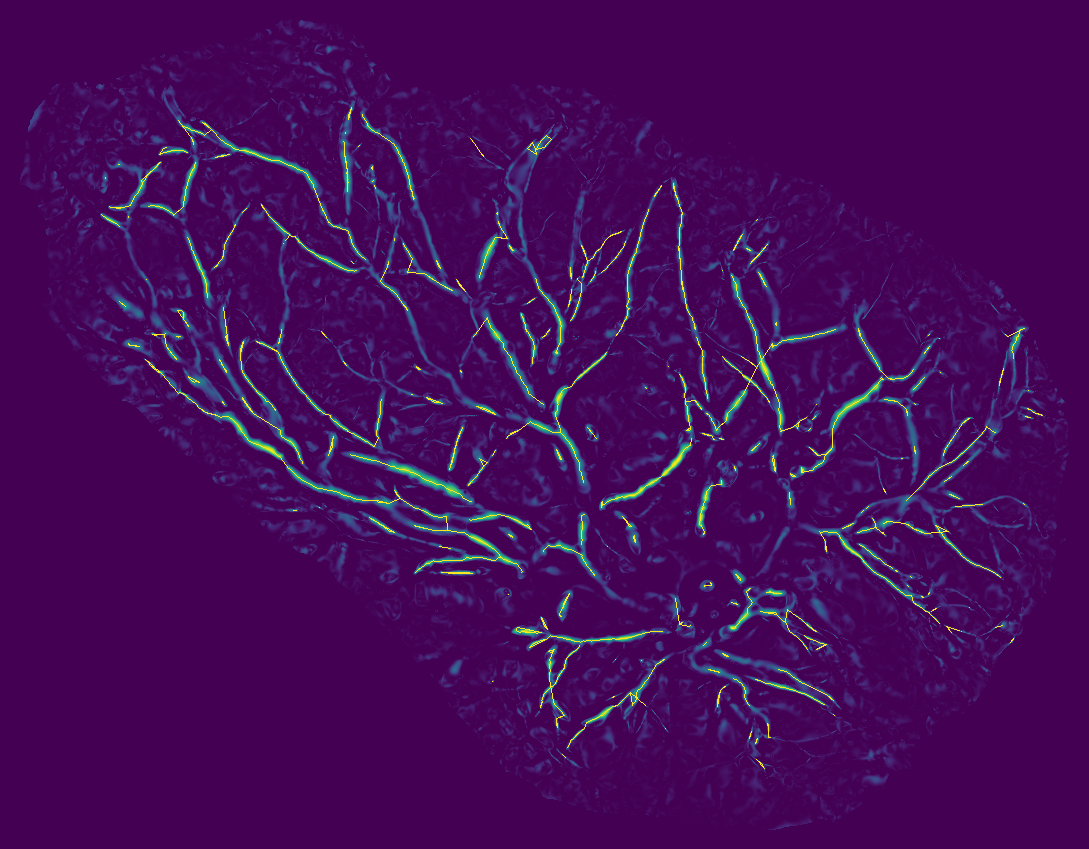
\includegraphics[height=0.4\textheight]{completed_by_nearest_to_line_mash}
	\caption{Partially completed network}
	\label{fig:network-completion-end-result}
\end{figure}

Finally, from the list of all remaining pairs of endpoints, we simply select the path along which the maximum mean value of $\Vmax$ is achieved. \cref{fig:network-completion-connected-pairs} shows non-violating paths between end-point pairs. The coloration shows the average value of $\Vmax$ along any straight path between compatible endpoints for which there does not occur any pixel with zero $\Vmax$. From these we can choose the path with largest average \Vmax. This partially completed network is shown in  \cref{fig:network-completion-end-result}(in yellow) overlaid on $\Vmax$.
We show this result as an indication of what can be done with the simple generation of $\Vmax$, although we simply demonstrate it here rather than including it in our main segmentation results. This is because, for its complexity, we hope we can instead solve both simple and predictive gap completion using a single method.

\begin{figure}[t] \centering
	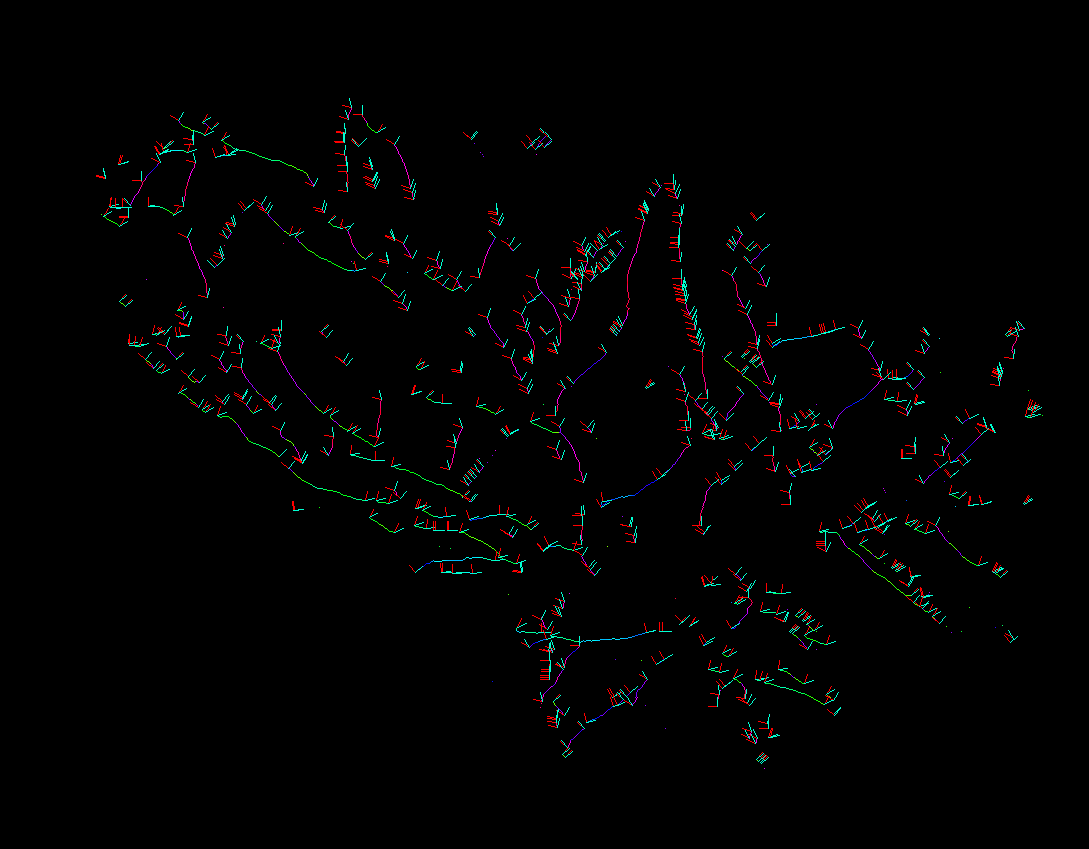
\includegraphics[width=0.8\linewidth]{pd_both}
	\caption{Approximated principal directions at endpoints}
	\label{fig:pd_demo}
\end{figure}

Finally, one final comment we can make. For the scale the maximum Frangi output occurs, at, we can look at the Hessian matrix itself to glean additional information. Recalling our discussion from \cref{ch:diffgeo}, we can instead of calculating the leading eigenvalue, we can calculate the leading \textit{eigenvector.} Just as the leading eigenvalue of the Hessian is a good approximation of the principal curvature at that point, the leading eigenvector is a good approximation of the principal direction. In \cref{fig:pd_demo} we show the vectors of the leading (and trailing) eigenvectors of each endpoint of the thinned, approximated network. We note that these could additionally be used towards the goal of network completion, but again we hesitate and instead look for a better overarching method that would address the gap problem.


\section{Further Research Directions}

Future research will first aim toward continue automating more of the preprocessing, specifically toward an even higher success rate of identifying the placental perimeter, umbilical cord insertion point, and any cuts without relying on a manual trace.  As mentioned in \cref{ch:research-protocol}, a more careful preparation of samples (i.e. as the picture is taken) would alleviate some of the difficulty of image registration. We also should improve our glare reduction algorithm, as it currently relies on an arbitrary threshold. We also need to remove the umbilical cord stump, as a large amount of noise around that point is still causing a large amount of noise in many samples. As far as our multiscale method goes, we would like to develop a notion of automatic scale selection, that would help us better normalize smaller scales, as well as allow us to find a specific largest scale (as some vessels in specific samples were only easily identified at very large scales, whereas these scales would introduce only noise in most other samples).
Finally, we strongly suggest further investigation of the usefulness of the Weingarten-based Frangi filter as compared to the convential Hessian-based one, as we briefly discussed in \cref{sec:wein-frangi}.

Any additional research on this problem that wishes to use the Frangi filter as a prefilter  (e.g. the trough completion method detailed in \cref{ch:segmentation} or some more involved algorithm) will likely need to solve the network completion problem, which we addressed briefly in \cref{sec:network-completion}.
